\documentclass[1p]{elsarticle_modified}
%\bibliographystyle{elsarticle-num}

%\usepackage[colorlinks]{hyperref}
%\usepackage{abbrmath_seonhwa} %\Abb, \Ascr, \Acal ,\Abf, \Afrak
\usepackage{amsfonts}
\usepackage{amssymb}
\usepackage{amsmath}
\usepackage{amsthm}
\usepackage{scalefnt}
\usepackage{amsbsy}
\usepackage{kotex}
\usepackage{caption}
\usepackage{subfig}
\usepackage{color}
\usepackage{graphicx}
\usepackage{xcolor} %% white, black, red, green, blue, cyan, magenta, yellow
\usepackage{float}
\usepackage{setspace}
\usepackage{hyperref}

\usepackage{tikz}
\usetikzlibrary{arrows}

\usepackage{multirow}
\usepackage{array} % fixed length table
\usepackage{hhline}

%%%%%%%%%%%%%%%%%%%%%
\makeatletter
\renewcommand*\env@matrix[1][\arraystretch]{%
	\edef\arraystretch{#1}%
	\hskip -\arraycolsep
	\let\@ifnextchar\new@ifnextchar
	\array{*\c@MaxMatrixCols c}}
\makeatother %https://tex.stackexchange.com/questions/14071/how-can-i-increase-the-line-spacing-in-a-matrix
%%%%%%%%%%%%%%%

\usepackage[normalem]{ulem}

\newcommand{\msout}[1]{\ifmmode\text{\sout{\ensuremath{#1}}}\else\sout{#1}\fi}
%SOURCE: \msout is \stkout macro in https://tex.stackexchange.com/questions/20609/strikeout-in-math-mode

\newcommand{\cancel}[1]{
	\ifmmode
	{\color{red}\msout{#1}}
	\else
	{\color{red}\sout{#1}}
	\fi
}

\newcommand{\add}[1]{
	{\color{blue}\uwave{#1}}
}

\newcommand{\replace}[2]{
	\ifmmode
	{\color{red}\msout{#1}}{\color{blue}\uwave{#2}}
	\else
	{\color{red}\sout{#1}}{\color{blue}\uwave{#2}}
	\fi
}

\newcommand{\Sol}{\mathcal{S}} %segment
\newcommand{\D}{D} %diagram
\newcommand{\A}{\mathcal{A}} %arc


%%%%%%%%%%%%%%%%%%%%%%%%%%%%%5 test

\def\sl{\operatorname{\textup{SL}}(2,\Cbb)}
\def\psl{\operatorname{\textup{PSL}}(2,\Cbb)}
\def\quan{\mkern 1mu \triangleright \mkern 1mu}

\theoremstyle{definition}
\newtheorem{thm}{Theorem}[section]
\newtheorem{prop}[thm]{Proposition}
\newtheorem{lem}[thm]{Lemma}
\newtheorem{ques}[thm]{Question}
\newtheorem{cor}[thm]{Corollary}
\newtheorem{defn}[thm]{Definition}
\newtheorem{exam}[thm]{Example}
\newtheorem{rmk}[thm]{Remark}
\newtheorem{alg}[thm]{Algorithm}

\newcommand{\I}{\sqrt{-1}}
\begin{document}

%\begin{frontmatter}
%
%\title{Boundary parabolic representations of knots up to 8 crossings}
%
%%% Group authors per affiliation:
%\author{Yunhi Cho} 
%\address{Department of Mathematics, University of Seoul, Seoul, Korea}
%\ead{yhcho@uos.ac.kr}
%
%
%\author{Seonhwa Kim} %\fnref{s_kim}}
%\address{Center for Geometry and Physics, Institute for Basic Science, Pohang, 37673, Korea}
%\ead{ryeona17@ibs.re.kr}
%
%\author{Hyuk Kim}
%\address{Department of Mathematical Sciences, Seoul National University, Seoul 08826, Korea}
%\ead{hyukkim@snu.ac.kr}
%
%\author{Seokbeom Yoon}
%\address{Department of Mathematical Sciences, Seoul National University, Seoul, 08826,  Korea}
%\ead{sbyoon15@snu.ac.kr}
%
%\begin{abstract}
%We find all boundary parabolic representation of knots up to 8 crossings.
%
%\end{abstract}
%\begin{keyword}
%    \MSC[2010] 57M25 
%\end{keyword}
%
%\end{frontmatter}

%\linenumbers
%\tableofcontents
%
\newcommand\colored[1]{\textcolor{white}{\rule[-0.35ex]{0.8em}{1.4ex}}\kern-0.8em\color{red} #1}%
%\newcommand\colored[1]{\textcolor{white}{ #1}\kern-2.17ex	\textcolor{white}{ #1}\kern-1.81ex	\textcolor{white}{ #1}\kern-2.15ex\color{red}#1	}

{\Large $\underline{11a_{151}~(K11a_{151})}$}

\setlength{\tabcolsep}{10pt}
\renewcommand{\arraystretch}{1.6}
\vspace{1cm}\begin{tabular}{m{100pt}>{\centering\arraybackslash}m{274pt}}
\multirow{5}{120pt}{
	\centering
	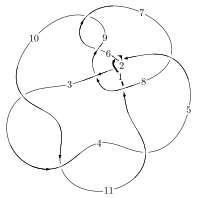
\includegraphics[width=112pt]{../../../GIT/diagram.site/Diagrams/png/400_11a_151.png}\\
\ \ \ A knot diagram\footnotemark}&
\allowdisplaybreaks
\textbf{Linearized knot diagam} \\
\cline{2-2}
 &
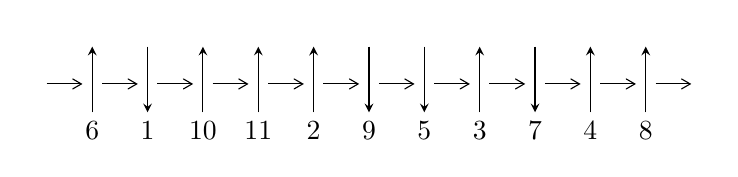
\begin{tikzpicture}[x=20pt, y=17pt]
	% nodes
	\node (C0) at (0, 0) {};
	\node (C1) at (1, 0) {};
	\node (C1U) at (1, +1) {};
	\node (C1D) at (1, -1) {6};

	\node (C2) at (2, 0) {};
	\node (C2U) at (2, +1) {};
	\node (C2D) at (2, -1) {1};

	\node (C3) at (3, 0) {};
	\node (C3U) at (3, +1) {};
	\node (C3D) at (3, -1) {10};

	\node (C4) at (4, 0) {};
	\node (C4U) at (4, +1) {};
	\node (C4D) at (4, -1) {11};

	\node (C5) at (5, 0) {};
	\node (C5U) at (5, +1) {};
	\node (C5D) at (5, -1) {2};

	\node (C6) at (6, 0) {};
	\node (C6U) at (6, +1) {};
	\node (C6D) at (6, -1) {9};

	\node (C7) at (7, 0) {};
	\node (C7U) at (7, +1) {};
	\node (C7D) at (7, -1) {5};

	\node (C8) at (8, 0) {};
	\node (C8U) at (8, +1) {};
	\node (C8D) at (8, -1) {3};

	\node (C9) at (9, 0) {};
	\node (C9U) at (9, +1) {};
	\node (C9D) at (9, -1) {7};

	\node (C10) at (10, 0) {};
	\node (C10U) at (10, +1) {};
	\node (C10D) at (10, -1) {4};

	\node (C11) at (11, 0) {};
	\node (C11U) at (11, +1) {};
	\node (C11D) at (11, -1) {8};
	\node (C12) at (12, 0) {};

	% arrows
	\draw[->,>={angle 60}]
	(C0) edge (C1) (C1) edge (C2) (C2) edge (C3) (C3) edge (C4) (C4) edge (C5) (C5) edge (C6) (C6) edge (C7) (C7) edge (C8) (C8) edge (C9) (C9) edge (C10) (C10) edge (C11) (C11) edge (C12) ;	\draw[->,>=stealth]
	(C1D) edge (C1U) (C2U) edge (C2D) (C3D) edge (C3U) (C4D) edge (C4U) (C5D) edge (C5U) (C6U) edge (C6D) (C7U) edge (C7D) (C8D) edge (C8U) (C9U) edge (C9D) (C10D) edge (C10U) (C11D) edge (C11U) ;
	\end{tikzpicture} \\
\hhline{~~} \\& 
\textbf{Solving Sequence} \\ \cline{2-2} 
 &
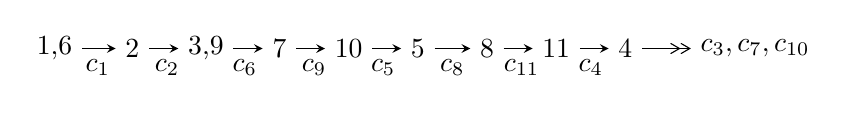
\begin{tikzpicture}[x=25pt, y=7pt]
	% node
	\node (A0) at (-1/8, 0) {1,6};
	\node (A1) at (1, 0) {2};
	\node (A2) at (33/16, 0) {3,9};
	\node (A3) at (25/8, 0) {7};
	\node (A4) at (33/8, 0) {10};
	\node (A5) at (41/8, 0) {5};
	\node (A6) at (49/8, 0) {8};
	\node (A7) at (57/8, 0) {11};
	\node (A8) at (65/8, 0) {4};
	\node (C1) at (1/2, -1) {$c_{1}$};
	\node (C2) at (3/2, -1) {$c_{2}$};
	\node (C3) at (21/8, -1) {$c_{6}$};
	\node (C4) at (29/8, -1) {$c_{9}$};
	\node (C5) at (37/8, -1) {$c_{5}$};
	\node (C6) at (45/8, -1) {$c_{8}$};
	\node (C7) at (53/8, -1) {$c_{11}$};
	\node (C8) at (61/8, -1) {$c_{4}$};
	\node (A9) at (10, 0) {$c_{3},c_{7},c_{10}$};

	% edge
	\draw[->,>=stealth]	
	(A0) edge (A1) (A1) edge (A2) (A2) edge (A3) (A3) edge (A4) (A4) edge (A5) (A5) edge (A6) (A6) edge (A7) (A7) edge (A8) ;
	\draw[->>,>={angle 60}]	
	(A8) edge (A9);
\end{tikzpicture} \\ 

\end{tabular} \\

\footnotetext{
The image of knot diagram is generated by the software ``\textbf{Draw programme}" developed by Andrew Bartholomew(\url{http://www.layer8.co.uk/maths/draw/index.htm\#Running-draw}), where we modified some parts for our purpose(\url{https://github.com/CATsTAILs/LinksPainter}).
}\phantom \\ \newline 
\centering \textbf{Ideals for irreducible components\footnotemark of $X_{\text{par}}$} 
 
\begin{align*}
I^u_{1}&=\langle 
5.94710\times10^{52} u^{65}+1.17236\times10^{53} u^{64}+\cdots+8.35081\times10^{52} b+2.54635\times10^{53},\\
\phantom{I^u_{1}}&\phantom{= \langle  }-8.47686\times10^{52} u^{65}-1.39894\times10^{53} u^{64}+\cdots+1.19297\times10^{52} a-2.19440\times10^{53},\;u^{66}+2 u^{65}+\cdots+4 u+1\rangle \\
I^u_{2}&=\langle 
u^2+7 b+6 u+4,\;- u^2+a- u-2,\;u^3+u^2+2 u+1\rangle \\
\\
\end{align*}
\raggedright * 2 irreducible components of $\dim_{\mathbb{C}}=0$, with total 69 representations.\\
\footnotetext{All coefficients of polynomials are rational numbers. But the coefficients are sometimes approximated in decimal forms when there is not enough margin.}
\newpage
\renewcommand{\arraystretch}{1}
\centering \section*{I. $I^u_{1}= \langle 5.95\times10^{52} u^{65}+1.17\times10^{53} u^{64}+\cdots+8.35\times10^{52} b+2.55\times10^{53},\;-8.48\times10^{52} u^{65}-1.40\times10^{53} u^{64}+\cdots+1.19\times10^{52} a-2.19\times10^{53},\;u^{66}+2 u^{65}+\cdots+4 u+1 \rangle$}
\flushleft \textbf{(i) Arc colorings}\\
\begin{tabular}{m{7pt} m{180pt} m{7pt} m{180pt} }
\flushright $a_{1}=$&$\begin{pmatrix}1\\0\end{pmatrix}$ \\
\flushright $a_{6}=$&$\begin{pmatrix}0\\u\end{pmatrix}$ \\
\flushright $a_{2}=$&$\begin{pmatrix}1\\- u^2\end{pmatrix}$ \\
\flushright $a_{3}=$&$\begin{pmatrix}u^2+1\\- u^2\end{pmatrix}$ \\
\flushright $a_{9}=$&$\begin{pmatrix}7.10566 u^{65}+11.7265 u^{64}+\cdots+31.4641 u+18.3944\\-0.712158 u^{65}-1.40388 u^{64}+\cdots-2.74081 u-3.04922\end{pmatrix}$ \\
\flushright $a_{7}=$&$\begin{pmatrix}8.72726 u^{65}+14.2298 u^{64}+\cdots+35.4678 u+22.1382\\-2.15625 u^{65}-3.59400 u^{64}+\cdots-6.93271 u-6.34045\end{pmatrix}$ \\
\flushright $a_{10}=$&$\begin{pmatrix}-5.31162 u^{65}-8.22686 u^{64}+\cdots-15.8436 u-12.2934\\3.63832 u^{65}+5.58995 u^{64}+\cdots+12.4635 u+8.35519\end{pmatrix}$ \\
\flushright $a_{5}=$&$\begin{pmatrix}- u\\u^3+u\end{pmatrix}$ \\
\flushright $a_{8}=$&$\begin{pmatrix}7.66328 u^{65}+12.2341 u^{64}+\cdots+30.8189 u+18.9851\\-1.32415 u^{65}-2.02616 u^{64}+\cdots-2.81894 u-3.05516\end{pmatrix}$ \\
\flushright $a_{11}=$&$\begin{pmatrix}-8.35519 u^{65}-13.0721 u^{64}+\cdots-33.0049 u-20.9573\\2.39639 u^{65}+3.80632 u^{64}+\cdots+8.95306 u+5.31162\end{pmatrix}$ \\
\flushright $a_{4}=$&$\begin{pmatrix}9.70575 u^{65}+15.5979 u^{64}+\cdots+36.1966 u+23.0110\\-3.81358 u^{65}-6.82103 u^{64}+\cdots-15.8119 u-9.70575\end{pmatrix}$\\ \flushright $a_{4}=$&$\begin{pmatrix}9.70575 u^{65}+15.5979 u^{64}+\cdots+36.1966 u+23.0110\\-3.81358 u^{65}-6.82103 u^{64}+\cdots-15.8119 u-9.70575\end{pmatrix}$\\&\end{tabular}
\flushleft \textbf{(ii) Obstruction class $= -1$}\\~\\
\flushleft \textbf{(iii) Cusp Shapes $= -8.99978 u^{65}-13.8805 u^{64}+\cdots-26.7379 u-16.3346$}\\~\\
\newpage\renewcommand{\arraystretch}{1}
\flushleft \textbf{(iv) u-Polynomials at the component}\newline \\
\begin{tabular}{m{50pt}|m{274pt}}
Crossings & \hspace{64pt}u-Polynomials at each crossing \\
\hline $$\begin{aligned}c_{1},c_{5}\end{aligned}$$&$\begin{aligned}
&u^{66}-2 u^{65}+\cdots-4 u+1
\end{aligned}$\\
\hline $$\begin{aligned}c_{2}\end{aligned}$$&$\begin{aligned}
&u^{66}+30 u^{65}+\cdots+2 u+1
\end{aligned}$\\
\hline $$\begin{aligned}c_{3},c_{4},c_{10}\end{aligned}$$&$\begin{aligned}
&u^{66}-2 u^{65}+\cdots- u^2-1
\end{aligned}$\\
\hline $$\begin{aligned}c_{6},c_{9}\end{aligned}$$&$\begin{aligned}
&u^{66}-4 u^{65}+\cdots+491 u-49
\end{aligned}$\\
\hline $$\begin{aligned}c_{7}\end{aligned}$$&$\begin{aligned}
&7(7 u^{66}-18 u^{65}+\cdots+13446 u-999)
\end{aligned}$\\
\hline $$\begin{aligned}c_{8}\end{aligned}$$&$\begin{aligned}
&7(7 u^{66}-10 u^{65}+\cdots+1391 u+241)
\end{aligned}$\\
\hline $$\begin{aligned}c_{11}\end{aligned}$$&$\begin{aligned}
&u^{66}-5 u^{65}+\cdots-3108 u+392
\end{aligned}$\\
\hline
\end{tabular}\\~\\
\newpage\renewcommand{\arraystretch}{1}
\flushleft \textbf{(v) Riley Polynomials at the component}\newline \\
\begin{tabular}{m{50pt}|m{274pt}}
Crossings & \hspace{64pt}Riley Polynomials at each crossing \\
\hline $$\begin{aligned}c_{1},c_{5}\end{aligned}$$&$\begin{aligned}
&y^{66}+30 y^{65}+\cdots+2 y+1
\end{aligned}$\\
\hline $$\begin{aligned}c_{2}\end{aligned}$$&$\begin{aligned}
&y^{66}+14 y^{65}+\cdots+14 y+1
\end{aligned}$\\
\hline $$\begin{aligned}c_{3},c_{4},c_{10}\end{aligned}$$&$\begin{aligned}
&y^{66}-62 y^{65}+\cdots+2 y+1
\end{aligned}$\\
\hline $$\begin{aligned}c_{6},c_{9}\end{aligned}$$&$\begin{aligned}
&y^{66}-36 y^{65}+\cdots-105155 y+2401
\end{aligned}$\\
\hline $$\begin{aligned}c_{7}\end{aligned}$$&$\begin{aligned}
&49(49 y^{66}+2434 y^{65}+\cdots-8.20438\times10^{7} y+998001)
\end{aligned}$\\
\hline $$\begin{aligned}c_{8}\end{aligned}$$&$\begin{aligned}
&49(49 y^{66}+880 y^{65}+\cdots-442127 y+58081)
\end{aligned}$\\
\hline $$\begin{aligned}c_{11}\end{aligned}$$&$\begin{aligned}
&y^{66}-21 y^{65}+\cdots-925904 y+153664
\end{aligned}$\\
\hline
\end{tabular}\\~\\
\newpage\flushleft \textbf{(vi) Complex Volumes and Cusp Shapes}
$$\begin{array}{c|c|c}  
\text{Solutions to }I^u_{1}& \I (\text{vol} + \sqrt{-1}CS) & \text{Cusp shape}\\
 \hline 
\begin{aligned}
u &= -0.886940 + 0.437138 I \\
a &= -1.43804 + 0.06126 I \\
b &= \phantom{-}0.278206 - 1.239240 I\end{aligned}
 & \phantom{-}6.34153 + 10.49840 I & \phantom{-}7.22778 - 5.33949 I \\ \hline\begin{aligned}
u &= -0.886940 - 0.437138 I \\
a &= -1.43804 - 0.06126 I \\
b &= \phantom{-}0.278206 + 1.239240 I\end{aligned}
 & \phantom{-}6.34153 - 10.49840 I & \phantom{-}7.22778 + 5.33949 I \\ \hline\begin{aligned}
u &= \phantom{-}0.900019 + 0.409306 I \\
a &= \phantom{-}1.287910 + 0.018413 I \\
b &= -0.259301 - 0.971541 I\end{aligned}
 & \phantom{-}0.06237 - 6.42817 I & \phantom{-0.000000 -}0. + 5.79651 I \\ \hline\begin{aligned}
u &= \phantom{-}0.900019 - 0.409306 I \\
a &= \phantom{-}1.287910 - 0.018413 I \\
b &= -0.259301 + 0.971541 I\end{aligned}
 & \phantom{-}0.06237 + 6.42817 I & \phantom{-0.000000 } 0. - 5.79651 I \\ \hline\begin{aligned}
u &= -0.301350 + 0.971582 I \\
a &= \phantom{-}1.01800 + 1.10633 I \\
b &= -0.559633 + 0.170616 I\end{aligned}
 & \phantom{-}0.012797 + 0.793621 I & \phantom{-0.000000 } 0 \\ \hline\begin{aligned}
u &= -0.301350 - 0.971582 I \\
a &= \phantom{-}1.01800 - 1.10633 I \\
b &= -0.559633 - 0.170616 I\end{aligned}
 & \phantom{-}0.012797 - 0.793621 I & \phantom{-0.000000 } 0 \\ \hline\begin{aligned}
u &= \phantom{-}0.372330 + 0.966152 I \\
a &= -0.71705 + 1.22172 I \\
b &= \phantom{-}0.635335 - 0.613059 I\end{aligned}
 & -4.16615 + 1.29044 I & \phantom{-0.000000 } 0 \\ \hline\begin{aligned}
u &= \phantom{-}0.372330 - 0.966152 I \\
a &= -0.71705 - 1.22172 I \\
b &= \phantom{-}0.635335 + 0.613059 I\end{aligned}
 & -4.16615 - 1.29044 I & \phantom{-0.000000 } 0 \\ \hline\begin{aligned}
u &= -0.789339 + 0.681407 I \\
a &= -0.170305 - 0.711151 I \\
b &= \phantom{-}0.612194 + 0.634929 I\end{aligned}
 & \phantom{-}1.79345 - 2.44057 I & \phantom{-0.000000 } 0 \\ \hline\begin{aligned}
u &= -0.789339 - 0.681407 I \\
a &= -0.170305 + 0.711151 I \\
b &= \phantom{-}0.612194 - 0.634929 I\end{aligned}
 & \phantom{-}1.79345 + 2.44057 I & \phantom{-0.000000 } 0\\
 \hline 
 \end{array}$$\newpage$$\begin{array}{c|c|c}  
\text{Solutions to }I^u_{1}& \I (\text{vol} + \sqrt{-1}CS) & \text{Cusp shape}\\
 \hline 
\begin{aligned}
u &= -0.893203 + 0.332658 I \\
a &= -1.067730 + 0.068534 I \\
b &= \phantom{-}0.060619 - 0.632472 I\end{aligned}
 & \phantom{-}0.93680 + 1.27321 I & \phantom{-}6.69528 - 2.55768 I \\ \hline\begin{aligned}
u &= -0.893203 - 0.332658 I \\
a &= -1.067730 - 0.068534 I \\
b &= \phantom{-}0.060619 + 0.632472 I\end{aligned}
 & \phantom{-}0.93680 - 1.27321 I & \phantom{-}6.69528 + 2.55768 I \\ \hline\begin{aligned}
u &= \phantom{-}0.010647 + 0.950386 I \\
a &= \phantom{-}0.878581 + 0.110969 I \\
b &= \phantom{-}0.018046 + 0.954751 I\end{aligned}
 & \phantom{-}4.00663 + 3.04870 I & \phantom{-}3.98275 - 2.96326 I \\ \hline\begin{aligned}
u &= \phantom{-}0.010647 - 0.950386 I \\
a &= \phantom{-}0.878581 - 0.110969 I \\
b &= \phantom{-}0.018046 - 0.954751 I\end{aligned}
 & \phantom{-}4.00663 - 3.04870 I & \phantom{-}3.98275 + 2.96326 I \\ \hline\begin{aligned}
u &= \phantom{-}0.861313 + 0.608674 I \\
a &= \phantom{-}0.420830 - 0.985449 I \\
b &= -1.035080 + 0.573403 I\end{aligned}
 & \phantom{-}7.36680 + 6.32316 I & \phantom{-0.000000 } 0 \\ \hline\begin{aligned}
u &= \phantom{-}0.861313 - 0.608674 I \\
a &= \phantom{-}0.420830 + 0.985449 I \\
b &= -1.035080 - 0.573403 I\end{aligned}
 & \phantom{-}7.36680 - 6.32316 I & \phantom{-0.000000 } 0 \\ \hline\begin{aligned}
u &= \phantom{-}0.538866 + 0.909098 I \\
a &= -0.472812 + 0.706075 I \\
b &= \phantom{-}5.56489 + 0.30058 I\end{aligned}
 & \phantom{-}3.51441 + 1.89915 I & \phantom{-0.000000 } 0 \\ \hline\begin{aligned}
u &= \phantom{-}0.538866 - 0.909098 I \\
a &= -0.472812 - 0.706075 I \\
b &= \phantom{-}5.56489 - 0.30058 I\end{aligned}
 & \phantom{-}3.51441 - 1.89915 I & \phantom{-0.000000 } 0 \\ \hline\begin{aligned}
u &= -0.477372 + 0.943179 I \\
a &= \phantom{-}0.324367 + 0.983761 I \\
b &= -1.73724 - 2.48467 I\end{aligned}
 & -2.01954 - 2.54235 I & \phantom{-0.000000 } 0 \\ \hline\begin{aligned}
u &= -0.477372 - 0.943179 I \\
a &= \phantom{-}0.324367 - 0.983761 I \\
b &= -1.73724 + 2.48467 I\end{aligned}
 & -2.01954 + 2.54235 I & \phantom{-0.000000 } 0\\
 \hline 
 \end{array}$$\newpage$$\begin{array}{c|c|c}  
\text{Solutions to }I^u_{1}& \I (\text{vol} + \sqrt{-1}CS) & \text{Cusp shape}\\
 \hline 
\begin{aligned}
u &= \phantom{-}0.706967 + 0.574992 I \\
a &= -0.344274 - 0.907805 I \\
b &= -0.497576 + 1.179170 I\end{aligned}
 & \phantom{-}2.68558 - 1.37819 I & \phantom{-}7.68512 + 2.61183 I \\ \hline\begin{aligned}
u &= \phantom{-}0.706967 - 0.574992 I \\
a &= -0.344274 + 0.907805 I \\
b &= -0.497576 - 1.179170 I\end{aligned}
 & \phantom{-}2.68558 + 1.37819 I & \phantom{-}7.68512 - 2.61183 I \\ \hline\begin{aligned}
u &= -0.742966 + 0.521978 I \\
a &= \phantom{-}0.391741 - 1.288390 I \\
b &= \phantom{-}0.73070 + 1.45249 I\end{aligned}
 & \phantom{-}9.13813 + 4.00163 I & \phantom{-}10.02198 - 1.95783 I \\ \hline\begin{aligned}
u &= -0.742966 - 0.521978 I \\
a &= \phantom{-}0.391741 + 1.288390 I \\
b &= \phantom{-}0.73070 - 1.45249 I\end{aligned}
 & \phantom{-}9.13813 - 4.00163 I & \phantom{-}10.02198 + 1.95783 I \\ \hline\begin{aligned}
u &= -0.422028 + 1.013150 I \\
a &= \phantom{-}0.42251 + 1.48918 I \\
b &= -1.47500 - 1.02933 I\end{aligned}
 & -0.83525 - 3.14253 I & \phantom{-0.000000 } 0 \\ \hline\begin{aligned}
u &= -0.422028 - 1.013150 I \\
a &= \phantom{-}0.42251 - 1.48918 I \\
b &= -1.47500 + 1.02933 I\end{aligned}
 & -0.83525 + 3.14253 I & \phantom{-0.000000 } 0 \\ \hline\begin{aligned}
u &= \phantom{-}0.490775 + 1.009750 I \\
a &= \phantom{-}0.050202 + 1.234540 I \\
b &= \phantom{-}1.73077 - 1.49983 I\end{aligned}
 & -3.33981 + 4.65284 I & \phantom{-0.000000 } 0 \\ \hline\begin{aligned}
u &= \phantom{-}0.490775 - 1.009750 I \\
a &= \phantom{-}0.050202 - 1.234540 I \\
b &= \phantom{-}1.73077 + 1.49983 I\end{aligned}
 & -3.33981 - 4.65284 I & \phantom{-0.000000 } 0 \\ \hline\begin{aligned}
u &= \phantom{-}0.496332 + 0.710814 I \\
a &= -0.254141 + 0.800937 I \\
b &= \phantom{-}0.81193 + 2.11193 I\end{aligned}
 & \phantom{-}4.10544 + 2.40688 I & \phantom{-}5.61601 - 0.93346 I \\ \hline\begin{aligned}
u &= \phantom{-}0.496332 - 0.710814 I \\
a &= -0.254141 - 0.800937 I \\
b &= \phantom{-}0.81193 - 2.11193 I\end{aligned}
 & \phantom{-}4.10544 - 2.40688 I & \phantom{-}5.61601 + 0.93346 I\\
 \hline 
 \end{array}$$\newpage$$\begin{array}{c|c|c}  
\text{Solutions to }I^u_{1}& \I (\text{vol} + \sqrt{-1}CS) & \text{Cusp shape}\\
 \hline 
\begin{aligned}
u &= -0.386686 + 0.758034 I \\
a &= \phantom{-}0.593747 + 0.711855 I \\
b &= \phantom{-}0.586006 + 1.214530 I\end{aligned}
 & -1.32206 - 1.19867 I & -0.30232 + 8.95765 I \\ \hline\begin{aligned}
u &= -0.386686 - 0.758034 I \\
a &= \phantom{-}0.593747 - 0.711855 I \\
b &= \phantom{-}0.586006 - 1.214530 I\end{aligned}
 & -1.32206 + 1.19867 I & -0.30232 - 8.95765 I \\ \hline\begin{aligned}
u &= -0.516301 + 1.034960 I \\
a &= -0.396217 + 1.250800 I \\
b &= -1.66301 - 1.61916 I\end{aligned}
 & \phantom{-}1.42288 - 7.01342 I & \phantom{-0.000000 } 0 \\ \hline\begin{aligned}
u &= -0.516301 - 1.034960 I \\
a &= -0.396217 - 1.250800 I \\
b &= -1.66301 + 1.61916 I\end{aligned}
 & \phantom{-}1.42288 + 7.01342 I & \phantom{-0.000000 } 0 \\ \hline\begin{aligned}
u &= -0.640786 + 0.965266 I \\
a &= -0.478037 + 0.069398 I \\
b &= -0.261638 - 0.444397 I\end{aligned}
 & \phantom{-}0.94099 - 2.93508 I & \phantom{-0.000000 } 0 \\ \hline\begin{aligned}
u &= -0.640786 - 0.965266 I \\
a &= -0.478037 - 0.069398 I \\
b &= -0.261638 + 0.444397 I\end{aligned}
 & \phantom{-}0.94099 + 2.93508 I & \phantom{-0.000000 } 0 \\ \hline\begin{aligned}
u &= \phantom{-}0.747809 + 0.382078 I \\
a &= \phantom{-}0.982939 + 0.436312 I \\
b &= \phantom{-}0.605214 - 0.686874 I\end{aligned}
 & \phantom{-}8.51869 + 1.38556 I & \phantom{-}10.68003 - 0.04077 I \\ \hline\begin{aligned}
u &= \phantom{-}0.747809 - 0.382078 I \\
a &= \phantom{-}0.982939 - 0.436312 I \\
b &= \phantom{-}0.605214 + 0.686874 I\end{aligned}
 & \phantom{-}8.51869 - 1.38556 I & \phantom{-}10.68003 + 0.04077 I \\ \hline\begin{aligned}
u &= \phantom{-}0.612668 + 1.023980 I \\
a &= \phantom{-}0.794130 + 0.357693 I \\
b &= \phantom{-}0.395162 - 1.268380 I\end{aligned}
 & \phantom{-}1.33847 + 6.45954 I & \phantom{-0.000000 } 0 \\ \hline\begin{aligned}
u &= \phantom{-}0.612668 - 1.023980 I \\
a &= \phantom{-}0.794130 - 0.357693 I \\
b &= \phantom{-}0.395162 + 1.268380 I\end{aligned}
 & \phantom{-}1.33847 - 6.45954 I & \phantom{-0.000000 } 0\\
 \hline 
 \end{array}$$\newpage$$\begin{array}{c|c|c}  
\text{Solutions to }I^u_{1}& \I (\text{vol} + \sqrt{-1}CS) & \text{Cusp shape}\\
 \hline 
\begin{aligned}
u &= \phantom{-}0.127139 + 0.784024 I \\
a &= -0.776775 + 0.573919 I \\
b &= -0.042614 + 0.780889 I\end{aligned}
 & -1.72069 - 1.07315 I & -1.43813 + 5.39557 I \\ \hline\begin{aligned}
u &= \phantom{-}0.127139 - 0.784024 I \\
a &= -0.776775 - 0.573919 I \\
b &= -0.042614 - 0.780889 I\end{aligned}
 & -1.72069 + 1.07315 I & -1.43813 - 5.39557 I \\ \hline\begin{aligned}
u &= -0.618729 + 1.050950 I \\
a &= -1.057990 + 0.338143 I \\
b &= -0.12777 - 1.65559 I\end{aligned}
 & \phantom{-}7.56649 - 9.18924 I & \phantom{-0.000000 } 0 \\ \hline\begin{aligned}
u &= -0.618729 - 1.050950 I \\
a &= -1.057990 - 0.338143 I \\
b &= -0.12777 + 1.65559 I\end{aligned}
 & \phantom{-}7.56649 + 9.18924 I & \phantom{-0.000000 } 0 \\ \hline\begin{aligned}
u &= -0.073346 + 1.249270 I \\
a &= -0.459853 - 0.956008 I \\
b &= -0.043571 + 0.947032 I\end{aligned}
 & \phantom{-}0.33897 + 7.84486 I & \phantom{-0.000000 } 0 \\ \hline\begin{aligned}
u &= -0.073346 - 1.249270 I \\
a &= -0.459853 + 0.956008 I \\
b &= -0.043571 - 0.947032 I\end{aligned}
 & \phantom{-}0.33897 - 7.84486 I & \phantom{-0.000000 } 0 \\ \hline\begin{aligned}
u &= \phantom{-}0.721856 + 1.027070 I \\
a &= \phantom{-}0.704898 - 0.295214 I \\
b &= -0.614618 - 0.468031 I\end{aligned}
 & \phantom{-}6.10958 - 0.48289 I & \phantom{-0.000000 } 0 \\ \hline\begin{aligned}
u &= \phantom{-}0.721856 - 1.027070 I \\
a &= \phantom{-}0.704898 + 0.295214 I \\
b &= -0.614618 + 0.468031 I\end{aligned}
 & \phantom{-}6.10958 + 0.48289 I & \phantom{-0.000000 } 0 \\ \hline\begin{aligned}
u &= \phantom{-}0.564876 + 1.135130 I \\
a &= -0.073078 - 0.707525 I \\
b &= -0.58777 + 1.86360 I\end{aligned}
 & \phantom{-}6.26544 + 3.61924 I & \phantom{-0.000000 } 0 \\ \hline\begin{aligned}
u &= \phantom{-}0.564876 - 1.135130 I \\
a &= -0.073078 + 0.707525 I \\
b &= -0.58777 - 1.86360 I\end{aligned}
 & \phantom{-}6.26544 - 3.61924 I & \phantom{-0.000000 } 0\\
 \hline 
 \end{array}$$\newpage$$\begin{array}{c|c|c}  
\text{Solutions to }I^u_{1}& \I (\text{vol} + \sqrt{-1}CS) & \text{Cusp shape}\\
 \hline 
\begin{aligned}
u &= \phantom{-}0.104431 + 1.298250 I \\
a &= \phantom{-}0.292746 - 0.847286 I \\
b &= -0.003012 + 0.940640 I\end{aligned}
 & -5.91703 - 3.42293 I & \phantom{-0.000000 } 0 \\ \hline\begin{aligned}
u &= \phantom{-}0.104431 - 1.298250 I \\
a &= \phantom{-}0.292746 + 0.847286 I \\
b &= -0.003012 - 0.940640 I\end{aligned}
 & -5.91703 + 3.42293 I & \phantom{-0.000000 } 0 \\ \hline\begin{aligned}
u &= -0.648304 + 1.133230 I \\
a &= -0.040925 - 1.149180 I \\
b &= \phantom{-}1.78851 + 1.92707 I\end{aligned}
 & \phantom{-}4.2340 - 16.1582 I & \phantom{-0.000000 } 0 \\ \hline\begin{aligned}
u &= -0.648304 - 1.133230 I \\
a &= -0.040925 + 1.149180 I \\
b &= \phantom{-}1.78851 - 1.92707 I\end{aligned}
 & \phantom{-}4.2340 + 16.1582 I & \phantom{-0.000000 } 0 \\ \hline\begin{aligned}
u &= \phantom{-}0.644245 + 1.145510 I \\
a &= \phantom{-}0.094859 - 1.051470 I \\
b &= -1.59384 + 1.71257 I\end{aligned}
 & -2.16297 + 12.09950 I & \phantom{-0.000000 } 0 \\ \hline\begin{aligned}
u &= \phantom{-}0.644245 - 1.145510 I \\
a &= \phantom{-}0.094859 + 1.051470 I \\
b &= -1.59384 - 1.71257 I\end{aligned}
 & -2.16297 - 12.09950 I & \phantom{-0.000000 } 0 \\ \hline\begin{aligned}
u &= -0.627293 + 1.165180 I \\
a &= -0.102093 - 0.901979 I \\
b &= \phantom{-}1.22622 + 1.56395 I\end{aligned}
 & -1.53699 - 6.84958 I & \phantom{-0.000000 } 0 \\ \hline\begin{aligned}
u &= -0.627293 - 1.165180 I \\
a &= -0.102093 + 0.901979 I \\
b &= \phantom{-}1.22622 - 1.56395 I\end{aligned}
 & -1.53699 + 6.84958 I & \phantom{-0.000000 } 0 \\ \hline\begin{aligned}
u &= -0.503518 + 0.347045 I \\
a &= \phantom{-}1.95488 - 0.23615 I \\
b &= -0.551149 + 1.270420 I\end{aligned}
 & \phantom{-}3.23237 + 2.81118 I & \phantom{-}6.49138 - 3.43190 I \\ \hline\begin{aligned}
u &= -0.503518 - 0.347045 I \\
a &= \phantom{-}1.95488 + 0.23615 I \\
b &= -0.551149 - 1.270420 I\end{aligned}
 & \phantom{-}3.23237 - 2.81118 I & \phantom{-}6.49138 + 3.43190 I\\
 \hline 
 \end{array}$$\newpage$$\begin{array}{c|c|c}  
\text{Solutions to }I^u_{1}& \I (\text{vol} + \sqrt{-1}CS) & \text{Cusp shape}\\
 \hline 
\begin{aligned}
u &= -0.263360 + 1.365470 I \\
a &= -0.207188 - 0.642987 I \\
b &= \phantom{-}0.127253 + 0.960247 I\end{aligned}
 & -4.52691 - 2.53329 I & \phantom{-0.000000 } 0 \\ \hline\begin{aligned}
u &= -0.263360 - 1.365470 I \\
a &= -0.207188 + 0.642987 I \\
b &= \phantom{-}0.127253 - 0.960247 I\end{aligned}
 & -4.52691 + 2.53329 I & \phantom{-0.000000 } 0 \\ \hline\begin{aligned}
u &= -0.427074\phantom{ +0.000000I} \\
a &= -0.433828\phantom{ +0.000000I} \\
b &= -0.336075\phantom{ +0.000000I}\end{aligned}
 & \phantom{-}0.801791\phantom{ +0.000000I} & \phantom{-}12.7100\phantom{ +0.000000I} \\ \hline\begin{aligned}
u &= \phantom{-}0.308392 + 0.295184 I \\
a &= -2.16318 + 0.94286 I \\
b &= \phantom{-}0.436188 + 0.731540 I\end{aligned}
 & -1.70503 - 0.88678 I & -1.07228 + 2.74548 I \\ \hline\begin{aligned}
u &= \phantom{-}0.308392 - 0.295184 I \\
a &= -2.16318 - 0.94286 I \\
b &= \phantom{-}0.436188 - 0.731540 I\end{aligned}
 & -1.70503 + 0.88678 I & -1.07228 - 2.74548 I \\ \hline\begin{aligned}
u &= -0.407213\phantom{ +0.000000I} \\
a &= \phantom{-}3.44853\phantom{ +0.000000I} \\
b &= -1.05852\phantom{ +0.000000I}\end{aligned}
 & \phantom{-}1.47039\phantom{ +0.000000I} & \phantom{-}6.43280\phantom{ +0.000000I}\\
 \hline 
 \end{array}$$\newpage\newpage\renewcommand{\arraystretch}{1}
\centering \section*{II. $I^u_{2}= \langle u^2+7 b+6 u+4,\;- u^2+a- u-2,\;u^3+u^2+2 u+1 \rangle$}
\flushleft \textbf{(i) Arc colorings}\\
\begin{tabular}{m{7pt} m{180pt} m{7pt} m{180pt} }
\flushright $a_{1}=$&$\begin{pmatrix}1\\0\end{pmatrix}$ \\
\flushright $a_{6}=$&$\begin{pmatrix}0\\u\end{pmatrix}$ \\
\flushright $a_{2}=$&$\begin{pmatrix}1\\- u^2\end{pmatrix}$ \\
\flushright $a_{3}=$&$\begin{pmatrix}u^2+1\\- u^2\end{pmatrix}$ \\
\flushright $a_{9}=$&$\begin{pmatrix}u^2+u+2\\-\frac{1}{7} u^2-\frac{6}{7} u-\frac{4}{7}\end{pmatrix}$ \\
\flushright $a_{7}=$&$\begin{pmatrix}u^2+u+2\\-\frac{1}{7} u^2+\frac{1}{7} u-\frac{4}{7}\end{pmatrix}$ \\
\flushright $a_{10}=$&$\begin{pmatrix}0\\- u\end{pmatrix}$ \\
\flushright $a_{5}=$&$\begin{pmatrix}- u\\- u^2- u-1\end{pmatrix}$ \\
\flushright $a_{8}=$&$\begin{pmatrix}\frac{4}{7} u^2+\frac{3}{7} u+\frac{9}{7}\\0\end{pmatrix}$ \\
\flushright $a_{11}=$&$\begin{pmatrix}1\\0\end{pmatrix}$ \\
\flushright $a_{4}=$&$\begin{pmatrix}u^2+1\\- u^2- u-1\end{pmatrix}$\\ \flushright $a_{4}=$&$\begin{pmatrix}u^2+1\\- u^2- u-1\end{pmatrix}$\\&\end{tabular}
\flushleft \textbf{(ii) Obstruction class $= 1$}\\~\\
\flushleft \textbf{(iii) Cusp Shapes $= \frac{204}{49} u^2+\frac{517}{49} u+\frac{368}{49}$}\\~\\
\newpage\renewcommand{\arraystretch}{1}
\flushleft \textbf{(iv) u-Polynomials at the component}\newline \\
\begin{tabular}{m{50pt}|m{274pt}}
Crossings & \hspace{64pt}u-Polynomials at each crossing \\
\hline $$\begin{aligned}c_{1}\end{aligned}$$&$\begin{aligned}
&u^3+u^2+2 u+1
\end{aligned}$\\
\hline $$\begin{aligned}c_{2}\end{aligned}$$&$\begin{aligned}
&u^3+3 u^2+2 u-1
\end{aligned}$\\
\hline $$\begin{aligned}c_{3},c_{4}\end{aligned}$$&$\begin{aligned}
&u^3+u^2-1
\end{aligned}$\\
\hline $$\begin{aligned}c_{5}\end{aligned}$$&$\begin{aligned}
&u^3- u^2+2 u-1
\end{aligned}$\\
\hline $$\begin{aligned}c_{6}\end{aligned}$$&$\begin{aligned}
&(u-1)^3
\end{aligned}$\\
\hline $$\begin{aligned}c_{7}\end{aligned}$$&$\begin{aligned}
&7(7 u^3+u^2-4 u+1)
\end{aligned}$\\
\hline $$\begin{aligned}c_{8}\end{aligned}$$&$\begin{aligned}
&7(7 u^3- u^2+u+1)
\end{aligned}$\\
\hline $$\begin{aligned}c_{9}\end{aligned}$$&$\begin{aligned}
&(u+1)^3
\end{aligned}$\\
\hline $$\begin{aligned}c_{10}\end{aligned}$$&$\begin{aligned}
&u^3- u^2+1
\end{aligned}$\\
\hline $$\begin{aligned}c_{11}\end{aligned}$$&$\begin{aligned}
&u^3
\end{aligned}$\\
\hline
\end{tabular}\\~\\
\newpage\renewcommand{\arraystretch}{1}
\flushleft \textbf{(v) Riley Polynomials at the component}\newline \\
\begin{tabular}{m{50pt}|m{274pt}}
Crossings & \hspace{64pt}Riley Polynomials at each crossing \\
\hline $$\begin{aligned}c_{1},c_{5}\end{aligned}$$&$\begin{aligned}
&y^3+3 y^2+2 y-1
\end{aligned}$\\
\hline $$\begin{aligned}c_{2}\end{aligned}$$&$\begin{aligned}
&y^3-5 y^2+10 y-1
\end{aligned}$\\
\hline $$\begin{aligned}c_{3},c_{4},c_{10}\end{aligned}$$&$\begin{aligned}
&y^3- y^2+2 y-1
\end{aligned}$\\
\hline $$\begin{aligned}c_{6},c_{9}\end{aligned}$$&$\begin{aligned}
&(y-1)^3
\end{aligned}$\\
\hline $$\begin{aligned}c_{7}\end{aligned}$$&$\begin{aligned}
&49(49 y^3-57 y^2+14 y-1)
\end{aligned}$\\
\hline $$\begin{aligned}c_{8}\end{aligned}$$&$\begin{aligned}
&49(49 y^3+13 y^2+3 y-1)
\end{aligned}$\\
\hline $$\begin{aligned}c_{11}\end{aligned}$$&$\begin{aligned}
&y^3
\end{aligned}$\\
\hline
\end{tabular}\\~\\
\newpage\flushleft \textbf{(vi) Complex Volumes and Cusp Shapes}
$$\begin{array}{c|c|c}  
\text{Solutions to }I^u_{2}& \I (\text{vol} + \sqrt{-1}CS) & \text{Cusp shape}\\
 \hline 
\begin{aligned}
u &= -0.215080 + 1.307140 I \\
a &= \phantom{-}0.122561 + 0.744862 I \\
b &= -0.149595 - 1.040080 I\end{aligned}
 & -4.66906 - 2.82812 I & -1.67995 + 11.45076 I \\ \hline\begin{aligned}
u &= -0.215080 - 1.307140 I \\
a &= \phantom{-}0.122561 - 0.744862 I \\
b &= -0.149595 + 1.040080 I\end{aligned}
 & -4.66906 + 2.82812 I & -1.67995 - 11.45076 I \\ \hline\begin{aligned}
u &= -0.569840\phantom{ +0.000000I} \\
a &= \phantom{-}1.75488\phantom{ +0.000000I} \\
b &= -0.129382\phantom{ +0.000000I}\end{aligned}
 & -0.531480\phantom{ +0.000000I} & \phantom{-}2.84970\phantom{ +0.000000I}\\
 \hline 
 \end{array}$$\newpage
\newpage\renewcommand{\arraystretch}{1}
\centering \section*{ III. u-Polynomials}
\begin{tabular}{m{50pt}|m{274pt}}
Crossings & \hspace{64pt}u-Polynomials at each crossing \\
\hline $$\begin{aligned}c_{1}\end{aligned}$$&$\begin{aligned}
&(u^3+u^2+2 u+1)(u^{66}-2 u^{65}+\cdots-4 u+1)
\end{aligned}$\\
\hline $$\begin{aligned}c_{2}\end{aligned}$$&$\begin{aligned}
&(u^3+3 u^2+2 u-1)(u^{66}+30 u^{65}+\cdots+2 u+1)
\end{aligned}$\\
\hline $$\begin{aligned}c_{3},c_{4}\end{aligned}$$&$\begin{aligned}
&(u^3+u^2-1)(u^{66}-2 u^{65}+\cdots- u^2-1)
\end{aligned}$\\
\hline $$\begin{aligned}c_{5}\end{aligned}$$&$\begin{aligned}
&(u^3- u^2+2 u-1)(u^{66}-2 u^{65}+\cdots-4 u+1)
\end{aligned}$\\
\hline $$\begin{aligned}c_{6}\end{aligned}$$&$\begin{aligned}
&((u-1)^3)(u^{66}-4 u^{65}+\cdots+491 u-49)
\end{aligned}$\\
\hline $$\begin{aligned}c_{7}\end{aligned}$$&$\begin{aligned}
&49(7 u^3+u^2-4 u+1)(7 u^{66}-18 u^{65}+\cdots+13446 u-999)
\end{aligned}$\\
\hline $$\begin{aligned}c_{8}\end{aligned}$$&$\begin{aligned}
&49(7 u^3- u^2+u+1)(7 u^{66}-10 u^{65}+\cdots+1391 u+241)
\end{aligned}$\\
\hline $$\begin{aligned}c_{9}\end{aligned}$$&$\begin{aligned}
&((u+1)^3)(u^{66}-4 u^{65}+\cdots+491 u-49)
\end{aligned}$\\
\hline $$\begin{aligned}c_{10}\end{aligned}$$&$\begin{aligned}
&(u^3- u^2+1)(u^{66}-2 u^{65}+\cdots- u^2-1)
\end{aligned}$\\
\hline $$\begin{aligned}c_{11}\end{aligned}$$&$\begin{aligned}
&u^3(u^{66}-5 u^{65}+\cdots-3108 u+392)
\end{aligned}$\\
\hline
\end{tabular}\newpage\renewcommand{\arraystretch}{1}
\centering \section*{ IV. Riley Polynomials}
\begin{tabular}{m{50pt}|m{274pt}}
Crossings & \hspace{64pt}Riley Polynomials at each crossing \\
\hline $$\begin{aligned}c_{1},c_{5}\end{aligned}$$&$\begin{aligned}
&(y^3+3 y^2+2 y-1)(y^{66}+30 y^{65}+\cdots+2 y+1)
\end{aligned}$\\
\hline $$\begin{aligned}c_{2}\end{aligned}$$&$\begin{aligned}
&(y^3-5 y^2+10 y-1)(y^{66}+14 y^{65}+\cdots+14 y+1)
\end{aligned}$\\
\hline $$\begin{aligned}c_{3},c_{4},c_{10}\end{aligned}$$&$\begin{aligned}
&(y^3- y^2+2 y-1)(y^{66}-62 y^{65}+\cdots+2 y+1)
\end{aligned}$\\
\hline $$\begin{aligned}c_{6},c_{9}\end{aligned}$$&$\begin{aligned}
&((y-1)^3)(y^{66}-36 y^{65}+\cdots-105155 y+2401)
\end{aligned}$\\
\hline $$\begin{aligned}c_{7}\end{aligned}$$&$\begin{aligned}
&2401(49 y^3-57 y^2+14 y-1)\\
&\cdot(49 y^{66}+2434 y^{65}+\cdots-82043766 y+998001)
\end{aligned}$\\
\hline $$\begin{aligned}c_{8}\end{aligned}$$&$\begin{aligned}
&2401(49 y^3+13 y^2+3 y-1)\\
&\cdot(49 y^{66}+880 y^{65}+\cdots-442127 y+58081)
\end{aligned}$\\
\hline $$\begin{aligned}c_{11}\end{aligned}$$&$\begin{aligned}
&y^3(y^{66}-21 y^{65}+\cdots-925904 y+153664)
\end{aligned}$\\
\hline
\end{tabular}
\vskip 2pc
\end{document}